\subsection{The Clock Synchronization Procedure}
\label{subsec:clock-sync-procedure}

\paragraph{Synchronization beacons.}
%
In the context of clock synchronization, we also call input-blocks as ``synchronization beacons'' (cf.~\cite{EC:BGKRZ21,TCC:GarKiaShe22}).
%
When parties are in the output generation (\textsf{OG}) stage of an interval \interval (in their local view), they mine beacons with their local time \protocolTime{\interval}{\round} and include all beacons (which are valid with respect to interval \interval) into their corresponding chains.
%
Note that beacons should still convey inputs for building the state machine (refer to~\cref{subsec:new-smr-protocol}) as well as local views of the previous interval to help retrieve the views and secure the parallel blockchain (\cref{subsec:new-parallel-blockchain}); for brevity we omit those details in this section.

Our shift calculation algorithm is based on comparing the timestamp recorded in beacons and their earliest local arrival time.
%
In order to perform such computation, parties need to bookkeep the time that they receive fresh beacons (in case parties receive duplicate beacons, they consider the one that arrives earliest in their local view).
%
Once a party \party receives a beacon \inputBlock (either directly or by observing it on a chain) at local time \protocolTime{\interval}{\round}, \party bookkeeps its arrival time in a local beacon registry $\mathsf{arrivalTime}(\cdot)$ as an entry $(\inputBlock, \protocolTime{\interval}{\round}, \mathrm{flag})$ where $\mathrm{flag} \in \{ \mathsf{temp}, \mathsf{final} \}$.
%
When the beacon \inputBlock is valid with respect to a fork in the parallel blocktrees in the current or previous interval, \party assigns \textsf{final} to the $\mathrm{flag}$ of \inputBlock; otherwise, it assigns \textsf{temp}.
%
Note that for a beacon \inputBlock labeled with \textsf{temp}, it will be removed from the registry when \party enters the corresponding interval and \party's local blockchain invalidates \inputBlock (invalid beacons are those that do not provide good fresh randomness with respect to any fork in party's local blocktrees).
%
Since timestamp is part of the block header, a beacon \inputBlock can be a valid one on multiple chains; yet, it suffices to bookkeep only one entry in $\mathsf{arrivalTime}(\cdot)$ and it can be reused for the same beacon in multiple chains.

A beacon \inputBlock is said to be \emph{valid} with respect to an interval $itvl$ and a chain \chain, if (i) \inputBlock reports a timestamp in the \textsf{OG} stage of interval $itvl$; (ii) \inputBlock points to the last block in the \textsf{VC} stage of interval $itvl$ on \chain; and (iii) \inputBlock is a valid PoW message w.r.t. $itvl$ and \chain.
%
Refer to~\cref{algorithm:isValidInputBlock} for a full description.

\paragraph{Shift calculation algorithm.}
%
We define $\mathsf{arrivalTime}$ as a function, taking a beacon \inputBlock as input, outputs its local arrival time \protocolTime{\interval}{\round}; recall that $\mathsf{TS}$ is a function that outputs the timestamp recorded in a block \block, we slightly abuse this notation and let it take also a beacon as input.
%
We write $\inputBlock \in \chain^{(i)}$ if a beacon \inputBlock is recorded in the output generation stage of $i$-th interval on a chain \chain and \inputBlock is valid with respect to \chain.
%
When the interval index is clear in the context, we drop the superscript and simply write $\inputBlock \in \chain$.

Parties compute a value \shift at the end of an interval (i.e., when their local clock enters a round such that $\round = (\interval - 1) \cdot \syncLen$), using beacons recorded in the current interval, and adds \shift to its local time.
%
Specifically, for a party \party with local parallel chains \parallelChainsLocal at the end of interval $itvl$, its local shift $\shift_\party$ is computed as
%
\begin{equation} \label{eq:sync-shift}
    \shift_\party
    \triangleq
    \mathsf{avg} \Big( \mathsf{select} \Big( \mathsf{reduce} \Big( \Big\{ \med \Big\{ \timestamp{\inputBlock} - \mathsf{arrivalTime}(\inputBlock) \mathbin\Big| \inputBlock \in \chain \Big\} \mathbin\Big| \chain \in \parallelChainsLocal \Big\}, \eta \Big), \eta \Big) \Big).
\end{equation}
%
where $\eta < m / 2$ is a protocol parameter, and \textsf{select} and \textsf{reduce} are as defined in~\cref{eq:reduce-select}.

Roughly speaking, this algorithm can be viewed as first adjusting a party \party's local clock separately on each single chains by computing the median shift (i.e., the difference between beacon time and its local receiving time) thus yielding $m$ different clock times; then, the same decision procedure as that in~\cref{protocol:approximate-consensus} is applied on these clocks, by filtering the largest and smallest $\eta$ ones, picking the first clock time every $\eta$ remaining values, and then compute their average.

With a positive \shift at the end of interval \interval, party \party skips \shift rounds and forward her local clock to \protocolTime{\interval + 1}{\interval \cdot \syncLen + \shift}.
%
Otherwise, her clock is set backward $|\shift|$ rounds and in the next round she tries to mine a block with timestamp \protocolTime{\interval + 1}{\interval \cdot \syncLen - |\shift|} for the $(itvl + 1)$-th interval.
%
Recall our timestamping scheme in~\cref{subsec:new-parallel-blockchain}, such ``retorted'' timestamp is allowed in the view convergence stage.
%
Additionally, parties will update their beacon registry, by applying \shift on the local receiving time of all future beacons.

We note that, with overwhelming probability, every \shift value that honest parties compute at the end of each interval is well-bounded, so that their logical time stays in a good linear envelope of the nominal time, which guarantees accuracy.
%
We also prove that, when parties start an interval with bounded skew $\initSkew = \bigTheta(\clockDrift \delay)$ and certain good properties on the parallel blockchains in this interval hold, after all honest parties enter the next interval, their local clocks are at most $\maxSkew = \bigTheta(\clockDrift \delay)$ apart from each other, which solves the synchronization problem.
%
Looking ahead, our full analysis (\cref{sec:full-protocol-analysis}) will show that these good properties hold throughout the entire execution and thus all intervals serve as good synchronizers.

\paragraph{The bootstrapping procedure.}
%
We now show how a fresh party, with total lack of knowledge other than the genesis block (CRS), can join the \pSMR protocol by passively observing the protocol execution for a \emph{constant} number of rounds.
%
We highlight that even without dynamic participation, this joining procedure is still of interest as parties that passively listening to the protocol can learn a precise time in the protocol and use it as a timestamping service.
%
This procedure also allows for an existing protocol participant, whose internal state suddenly gets flushed, to catch-up with other honest parties.

Consider a newly joining party \newParty.
%
Given the interval retrieval mechanism introduced in~\cref{subsec:new-parallel-blockchain}, \newParty can bootstrap her local parallel blocktrees \parallelTreesLocal, by listening to the protocols for a constant amount of time and updating the heaviest chain such that for each interval, \newParty obliviously learns a subset of forks that are in the common view of alert parties.
%
Nonetheless, recall our timestamping scheme in~\cref{subsec:new-parallel-blockchain}, blockchains only provide a coarse notion of time such that the local clock of \newParty can deviate from alert ones for $\syncLen_{\mathsf{VC}}$ rounds.
%
Our goal is to further tighten this skew to $\maxSkew = \bigTheta(\clockDrift \delay)$ --- a small constant.

We now explain how the fresh party \newParty can synchronize with alert parties with well-bounded skews.
%
Upon executing the bootstrapping procedure, \newParty resets her local clock to \protocolTime{1}{1}.
%
During the bootstrapping phase, \newParty also listens to the beacon diffusion network $\funcDiffuse^{\textsf{input}}$ and bookkeep the arrival time of all beacons.
%
This phase lasts for more than two interval durations so that \newParty observes at least one complete output generation stage in an interval.
%
Since \newParty is not synchronized, she cannot filter any invalid beacons so she temporarily mark all beacons as \textsf{temp}.
%
Nonetheless, after she finishes bootstrapping her parallel blockchain, \newParty roughly understands which interval she stays in hence \newParty starts to remove invalid beacons based on her local heaviest chain.
%
Note that our protocol guarantees that a large fraction of chains yield good properties at the end of an interval (e.g., common view of the chain in the output generation stage), \newParty thus shares the same beacon set (marked as \textsf{final}) with alert parties on sufficiently many chains.
%
At the end of the bootstrapping procedure, by iterating all complete intervals that \newParty has observed and applying sequentially the shift calculation algorithm in~\cref{eq:sync-shift}, \newParty synchronizes her clock with all alert parties.
%
Note that when \newParty has observed two or more complete intervals, the local arrival time of all beacons in the second and later intervals needs to be updated each time after clock adjustment, by adding shift computed from the last interval to these beacons.
%
The full description of the bootstrapping procedure is presented in~\cref{protocol:joining-procedure}.

\paragraph{An improved honest-majority lower bound for clock synchronization.}
%
We discuss under what circumstances honest majority is necessary for clock synchronization.
%
Regarding corruption resiliency of synchronization problems, in the information-theoretic setting, Dolev \textit{et al.} \cite{JCSS:DHS86} show that clock synchronization is impossible when more than one-third of the parties are corrupted.
%
In the authenticated setting (assuming unforgeable signatures and a PKI), on one side, Srikanth and Toueg \cite{JACM:SriTou87} show that honest majority is necessary when the resulting linear envelope on logical time is as good as that on nominal time.
%
On the other side, Halpern \textit{et al.} \cite{PODC:HSSD84} presents a dishonest majority protocol however its logical time can deviate drastically from the real time as the number of corrupted parties grows.

We extend the argument for honest majority in~\cite{JACM:SriTou87} to a more general accuracy condition.
%
In a nutshell, when physical clocks drifts in a $(1 + \clockDrift)$-linear envelope, we show that to stay in the time that is \emph{strictly tighter} than a $(1 + \clockDrift)^2$-linear envelope of nominal time, a majority of honest parties (resources) is necessary.
%
We state this result in~\cref{thm:honest-majority-necessity}, and a depiction on the logical linear envelope where honest majority is necessary can be found in~\cref{fig:honest-majority}.

\begin{figure}[ht] \centering
    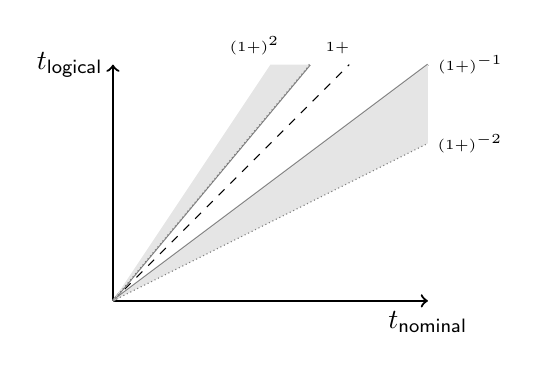
\begin{tikzpicture}
        \draw[->, thick] (0, 0) -- (4, 0) node[below] {$t_{\mathsf{nominal}}$};
        \draw[->, thick] (0, 0) -- (0, 3) node[left] {$t_{\mathsf{logical}}$};
        \draw[dashed] (0, 0) -- (3, 3);

        \draw[thick, color = gray] (0, 0) -- (4, 3) node[right, color = black] {\tiny $(1 + \clockDrift)^{-1}$};

        \draw[thick, color = gray] (0, 0) -- (2.5, 3) node[above, color = black, xshift = 1em] {\tiny $1 + \clockDrift$};

        \fill[fill = gray!20] (0, 0) -- (4, 3) -- (4, 2);
        \fill[fill = gray!20] (0, 0) -- (2, 3) -- (2.5, 3);

        \draw[densely dotted, color = gray] (0, 0)--(4, 2) node[right, color = black] {\tiny $(1 + \clockDrift)^{-2}$};
        \draw[densely dotted, color = gray] (0, 0)--(2.5, 3) node[above, color = black, xshift = -2em] {\tiny $(1 + \clockDrift)^2$};
    \end{tikzpicture}
    \caption{\sl An illustration of the logical time linear envelope (in gray) such that honest majority is necessary.}
    \label{fig:honest-majority}
\end{figure}


\begin{theorem} \label{thm:honest-majority-necessity}
    Any clock synchronization protocol run by parties with \clockDrift-linear-envelope physical clocks that achieves \maxSkew-bounded skews and $\varGamma$-accuracy such that $\maxSkew \in \mathbb{N}$ and $\clockDrift \le \varGamma < 2\clockDrift + \clockDrift^2$ must have a majority of honest parties.
\end{theorem}

\begin{proof}
    Let $D_i(r)$ denote the clock of party $\party_i$ at nominal time $r$ and $C_i(r)$ denote the (exported) logical time of party $\party_i$ at nominal time $r$.

    Assume $0 < \epsilon \ll \clockDrift$ and there exists a protocol that achieves  $((1 + \clockDrift)^{-1} (1 + \clockDrift - \epsilon)^{-1}, (1 + \clockDrift) (1 + \clockDrift - \epsilon))$-accuracy with dishonest majority.
    %
    We show that it is impossible by first considering a system with two parties $\party, \party'$ and the following three executions.
    %
    \begin{cccItemize}[noitemsep]
        \item \emph{Execution $E_1$.}
        %
        Both the parties follow the protocol, and party \party has the maximum clock speed (i.e., $D_1(r) = (1 + \clockDrift) r$); party $\party'$ has the minimum speed ($D'_1(r) = (1 + \clockDrift)^{-1} r$).
        %
        Moreover, all messages have delay exactly $\delay / (1 + \clockDrift)^2$.

        \item \emph{Execution $E_2$.}
        %
        Party \party is honest and has rate $R_2(r) = (1 + \clockDrift)^{-1} r$; party $\party'$ is corrupted and runs at $R'_2(r) = (1 + \clockDrift)^{-3} r$ but is otherwise correct.
        %
        Moreover, all messages have delay exactly \delay.

        \item \emph{Execution $E_3$.}
        %
        Party $\party'$ is honest and has rate $R'_3(r) = (1 + \clockDrift) r$; party $\party_1$ is corrupted and runs at $R_3(r) = (1 + \clockDrift)^3 r$ but is otherwise correct.
        %
        Moreover, all messages have delay exactly $\delay / (1 + \clockDrift)^4$.
    \end{cccItemize}
    %
    All these three executions follow the clock and network assumptions and are hence admissible.
    %
    In addition, executions $E_1$ and $E_2$ are indistinguishable for party \party; and executions $E_1$ and $E_3$ are indistinguishable for party $\party'$.
    %
    Since accuracy is achieved, \party in execution $E_1$ will report a time $C_1(r) \le (1 + \clockDrift)(1 + \clockDrift - \epsilon) r + b_1$.
    %
    Since $D_1(r) = (1 + \clockDrift) r$, we find that $C_1(r) \le (1 + \clockDrift - \epsilon) D_1(r) + b^1$.
    %
    Similarly, by considering execution $E_2$ we have $(1 + \clockDrift - \epsilon)^{-1} C_2(r) + a_2 \le C_2(r)$.
    %
    Since executions $E_1$ and $E_2$ are indistinguishable for party \party, the relation between its exported time and reading time must be the same in both executions.
    %
    Therefore, we have for $k = 1, 2$,
    %
    \[ (1 + \clockDrift - \epsilon)^{-1} D_k(r) + a_2 \le C_k(r) \le (1 + \clockDrift - \epsilon) D_k(r) + b_1. \]
    %
    I.e., in execution $E_1$ we can find a time $\tau_1$ such that for all $r > \tau_1$,
    %
    \[ (1 + \clockDrift - \epsilon)^{-1} (1 + \clockDrift) r + a_2 \le C_1(r) \le (1 + \clockDrift - \epsilon) (1 + \clockDrift) r + b_1. \]
    %
    Similarly, by considering party $\party'$ in executions $E_1$ and $E_3$, we see that there exist a time $\tau_2$ in execution $E_1$ such that for all $r > \tau_2$,
    %
    \[ (1 + \clockDrift - \epsilon)^{-1} (1 + \clockDrift)^{-1} r + a_1 \le C'_1(r) \le (1 + \clockDrift - \epsilon) (1 + \clockDrift)^{-1} r + b_3. \]
    %
    Hence, we find that there exist a time $\tau \ge \max \{ \tau_1, \tau_2 \}$ in execution $E_1$ such that for all $r > \tau$, the deviation between the exported time of two correct parties is greater than a constant \maxSkew, which violates the bounded skew condition.
\end{proof}
